% set the document type and base font size
\documentclass[17pt]{extarticle}

% Geometry package supports custom border and format definitions
\usepackage[a4paper, top=2cm, bottom=2cm, left=2cm, right=2cm]{geometry}
% extsizes package allows to set the base font size to 8-20 pixels (https://ctan.org/pkg/extsizes)
\usepackage{extsizes}
% remove limitation to ascii by introducing UTF8 support 
\usepackage[utf8]{inputenc}
% enables support for the german 'Umlaute': ä, ö, ü
\usepackage[T1]{fontenc}
% mathematical expressions with tabstop support (https://texblog.org/2008/10/01/adding-normal-text-into-formulas/)
\usepackage{amsmath}
% text coloring, obviously
\usepackage{color}
% import and positioning of pictures and graphics
\usepackage{graphicx}

% disable indentation for new paragraphs
\setlength{\parindent}{0pt}

% document meta information
\author{Lukas Steiger}
\title{HSR Formelsammlung PhAI}
\date{20.4.17}

% start of the document content
\begin{document}
\begin{center}
	\huge{HSR Formelsammlung PhAI} \\
	\small{Autor: Lukas Steiger}
\end{center}
	
\section{Grundlagen - Bewegung und Kräfte}

	Geschwindigkeit
	\begin{align}
		v = v_{0} * a * t
	\end{align}
	
	Kraft \small{(Newtonsches Bewegungsgesetz)}
	\begin{align}
		&F = m * a
		&&F = m * g
	\end{align}
	
	Schwerkraft \small{(Gravitationskraft)}
	\begin{align}
		&F_{G} = m * g
		&&g = 9.81 \frac{m}{s^{2}} 
	\end{align}
	
	Zurückgelegte Strecke \small{($s_{0}$ oder $v_{0}*t$ weglassen, falls 0)}
	\begin{align}
		&s(t) = s_{0} + v_{0} * t + \frac{a}{2} * t^{2}
		&&\text{\small{oder einfach}}
		&&&s = v * t
	\end{align}

	\subsection{Würfe}

	\subsubsection{Senkrechter Wurf}
	\begin{align}
		y * v_{0} * t - \frac{g}{2} * t^{2}
	\end{align}
	
	Wurfhöhe
	\begin{align}
		h = \frac{v_{0}^{2}}{2g}
	\end{align}
	
	\subsubsection{Horizontaler Wurf}
	\begin{align}
		y = - \frac{g}{2v_{0}^{2}} * x^{2}
	\end{align}
	
	Wurfweite
	\textcolor{red}{Gibts da eine Formel?}
	
	\subsubsection{Schiefer Wurf}
	\begin{align}
		y(x) = x * \tan \varphi - \frac{g}{2 * v_{0}^{2} * \cos^{2} \varphi} * x^{2}
	\end{align}
	
	Wurfhöhe
	\begin{align}
		y_{max} = \frac{v_{0}^{2} * \sin^{2} \varphi}{2g}
	\end{align}
	
	Wurfweite
	\begin{align}
		d = \frac{v_{0}^{2} * \sin(2\varphi)}{g}
	\end{align}

\section{Kräfte, Arbeit, Leistung \& Energie}
	\begin{figure}[h!]
		\centering
		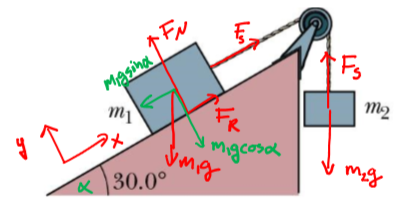
\includegraphics[width=8cm]{./img/Haftreibung.png}
	\end{figure}
	
	Normalkraft
	\begin{align}
		\textcolor{red}{TODO}
	\end{align}
	
	Maximale Haftreibung
	\begin{align}
		&F_{R,max} = \mu_{H} * F_{N}
		&&\mu_{H} = \text{Haftreibungskoeffizient} 
	\end{align}

	Konstante Gleitreibung
	\begin{align}
		&F = \mu_{G} * F_{N}
		&&\mu_{G} = \text{Gleitreibungskoeffizient}		
	\end{align}

	Mechanische Arbeit \small{($1J = 1Nm = \frac{1*kg m^{2}}{s^{2}}$)}
	\begin{align}
		&W = F * s 
		&&W = m * g * h = \varrho * V * m * g
	\end{align}

	Energieerhaltung
	\begin{align}
		E_{pot} + E_{kin} = \text{konstant}
	\end{align}
	
	Potentielle Energie
	\begin{align}
		&\text{geleistete Arbeit} 
		&&W = E_{pot} 
		&&&\text{potentielle Energie}
	\end{align}
	
	Kinetische Energie
	\begin{align}
		E_{kin} = \frac{1}{2} * m * v^{2}
	\end{align}
	
	Federenergie
	\begin{align}
		&E_{pot} = \frac{1}{2} * k * x^{2}
		&&k = \textcolor{red}{WAS??}
		&&&x = \text{Ausdehnung Feder}
	\end{align}
	
	Leistung \small(Arbeit pro Zeiteinheit in $J/s$)
	\begin{align}
		P = F * v = m * a^{2} * t
	\end{align}
	
	Impuls / Gesamtimpuls
	\begin{align}
		&p = m * v
		&&P = p_{1} + p_{2} + ... + p_{n}
	\end{align}
	
	Schwerpunktgeschwindigkeit
	\begin{align}
		u = \frac{p_{1} + p_{2} + ... + p_{n}}{m_{1} + m_{2} + ... + m_{n}}
	\end{align}
	
\section{Repetition - Trigonometrie}
	\begin{align}
		&\sin \alpha = \frac{a}{c}
		&&\cos \alpha = \frac{b}{c}
		&&&\tan \alpha = \frac{a}{b}
	\end{align}
	\begin{figure}[h!]
		\centering
		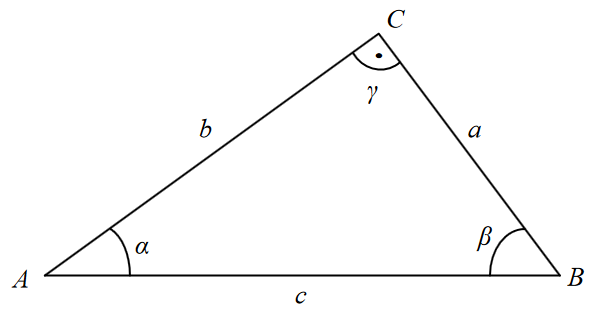
\includegraphics[width=10cm]{./img/Trigonometrie.png}
	\end{figure}

\section{ToDo's}
	\color{red}
	\begin{itemize}
		\item All de Integral Gugus vo SW02
		\item Relative/tatsächliche Beschleunigung/Geschwindigkeit (SW02)
		\item Kreisbewegung, Winkelgeschwindigkeit (SW02)
		\item Drehmoment ... (SW07?)
		\item Alles wo mer nanig gha hend :-)
	\end{itemize}
\end{document}
